\documentclass[twocolumn]{IEEEtran}
\usepackage{graphicx} % Required for inserting images
\usepackage{flushend}
\usepackage{float}
\usepackage{geometry}
\usepackage{amsmath}
\usepackage{color}
\usepackage[hidelinks]{hyperref} % 超链接
\usepackage{subcaption} % 用于创建子图和子标题
\usepackage{booktabs} % For professional looking tables
\usepackage{setspace} % 设置行间距
\geometry{a4paper,scale=0.85}

\title{CW2 Lab Report}  
\author{Name: Junhao Huang \and Student ID: 2256793 \and TA: Yu Kang} 
\date{\today}  

\begin{document}
% \onehalfspacing  % 设置1.5倍行距

\maketitle

% 介绍
\section{Introduction}
% 基础介绍
\subsection{Basic Information}
After the original student information data cleaning and dimensionalization reduction, different classifier methods will be trained and tested in this experiment, and students will be classified according to the program to which each student belongs. For different classification algorithms, the proportion of training set of each classifier is adjusted to 70\%, and \textbf{five-fold cross-validation} is applied to the initial classification results, that is, the original delimit training set is re-divided into 5 subsets, and then one group is selected in turn for training, reducing the model's dependence on specific data samples. The content outside of each subset is then treated as a test set, and using a different test set each time also makes the data learned by the model more extensive. Since dimensionality reduction results in a loss of data information, the following categories will be trained directly using the raw data. Finally, F1 Score and accuracy are obtained according to the classifier.

% F1 score公式
\begin{equation}
    F1 = 2 \times \frac{\text{Precision} \times \text{Recall}}{\text{Precision} + \text{Recall}}
\end{equation}
\textit{F1 score is the harmonic mean of Precision and Recall}

Finally, the classification effectiveness will be evaluated based on the \textbf{F1 score} obtained from the classifier.

% 分类器选择介绍
\subsection{Classifier Selection}
In this article, the \textbf{single decision tree} and the \textbf{random forest} of multiple decision arrays will be used to analyze each decision tree. Then, a \textbf{support vector machine (SVM)} is used to find the best model configuration of the SVM with the selected feature set to precisely classify the student's course. \textbf{SVM is known for its effectiveness in handling high-dimensional data and nonlinear relationships, so it is expected that SVM will be more competent for this task.} The naive Bayes classifier will then be used, since naive Bayes is a probabilistic classifier that assumes that features are independent from each other, understanding its behavior under different feature sets will be important for model optimization. Finally, an ensemble learning method classifier will be built, which brings together the basic classifiers of decision tree, SVM and naive Bayes to improve classification accuracy.

% 特征选择
\subsection{Features Set Selection}
The first step is to determine how to select the appropriate feature set for training the classifier model. The original data table contains \textbf{11 features}, and by first observing these features, you can notice that 'Index' is only self-numbered, not valid data, because it can be removed first. Then, since different programmes of students need to be classified, programmes also need to be extracted. For the rest of the 9 characteristics \textbf{[``Grade", ``Gender", ``Total", ``MCQ, ``Q1'', ``Q2'', ``Q3'', ``Q4'', ``Q5'']}, the first nine feature combination as a set of feature set. The \textbf{Recursive Feature Elimination with Cross-Validation (RFECV)} method is then used, a powerful automatic feature selection method that combines recursive feature elimination and cross-validation to automatically determine the optimal feature set for model training. Here, I will first separate the content corresponding to the features of the original Programme into four groups of target variables: Programme1-Programme4, and then evaluate the importance of the features of these four categories respectively, and finally determine the most effective feature set corresponding to each category. The judgment result is that the 8 features \textbf{[``Grade'', ``Total'', ``MCQ'', ``Q1'', ``Q2'',``Q3'', ``Q4'', ``Q5'']} have the greatest overall influence, so these eight features are also grouped into a feature set.
% 每个分类对应的最佳特征集
\begin{table}[H]
    \centering
    {\small % 设置字体大小为small
    \begin{tabular}{|c|c|p{3.5cm}|} % 缩小表格的总体宽度
    \hline
    \textbf{Programme} & \textbf{Optimal} & \textbf{Features to Keep} \\
        \hline
        P1 & 8 & Grade, Total, MCQ, Q1, Q2, Q3, Q4, Q5 \\
        \hline
        Pd & 7 & Total, MCQ, Q1, Q2, Q3, Q4, Q5 \\
        \hline
        P3 & 1 & Grade \\
        \hline
        P4 & 8 & Gender, Total, MCQ, Q1, Q2, Q3, Q4, Q5 \\
        \hline
    \end{tabular}
    } % 结束字体大小设置
\end{table}

\textit{The optimal set of features obtained from 4 different Programme classifications}

Finally, the method of random forest is used to judge the feature set that has the greatest impact on the classification, and the optimal selection is \textbf{[``Total'', ``Grade'', ``Q1'', ``Q4'']}, and it is regarded as the third feature set.

\section{Decision Tree}
\subsection{Single Decision Tree}
In the classification task, the decision tree makes predictions by learning the mapping relationship between the input feature and the output category, each node in the decision tree represents a feature, and the branch represents the class assignment based on the feature condition. By traversing from the root node to the leaf nodes of the tree, the final classification result can be obtained. However, in the decision number, in order to ensure the best results, the effectiveness of root node classification is very important. In this experiment, \textbf{Gini coefficient} is used to judge the best split points and nodes of each segment.
% 基尼指数的公式
\begin{equation}
    Gini(t) = 1 - \sum_{i=1}^k p_i^2
\end{equation}
\textit{Where \(p_i^2 \) represents the probability that the randomly selected sample is correctly classified. Thus, \(1 - \sum_{i=1}^k p_i^2 \) represents the probability that there is at least one classification error, namely the impurity of the node. The smaller the Gini coefficient value, the higher the purity of the node}

Gini coefficient can reduce the complexity of the model according to the purity and specify pruning strategies to limit the growth of the tree, so as to prevent overfitting of the model, because if the number is allowed to grow unrestricted, the results obtained by the decision tree can only be applied to the training set and the generalization ability on the unknown data is poor, especially for the data of this experiment, the amount of data is not large. It is very likely that the classifier will only judge the rules of the training set, leading to overfitting.

% 决策树图像
\begin{figure}[H]
    \centering % 使图片居中显示
    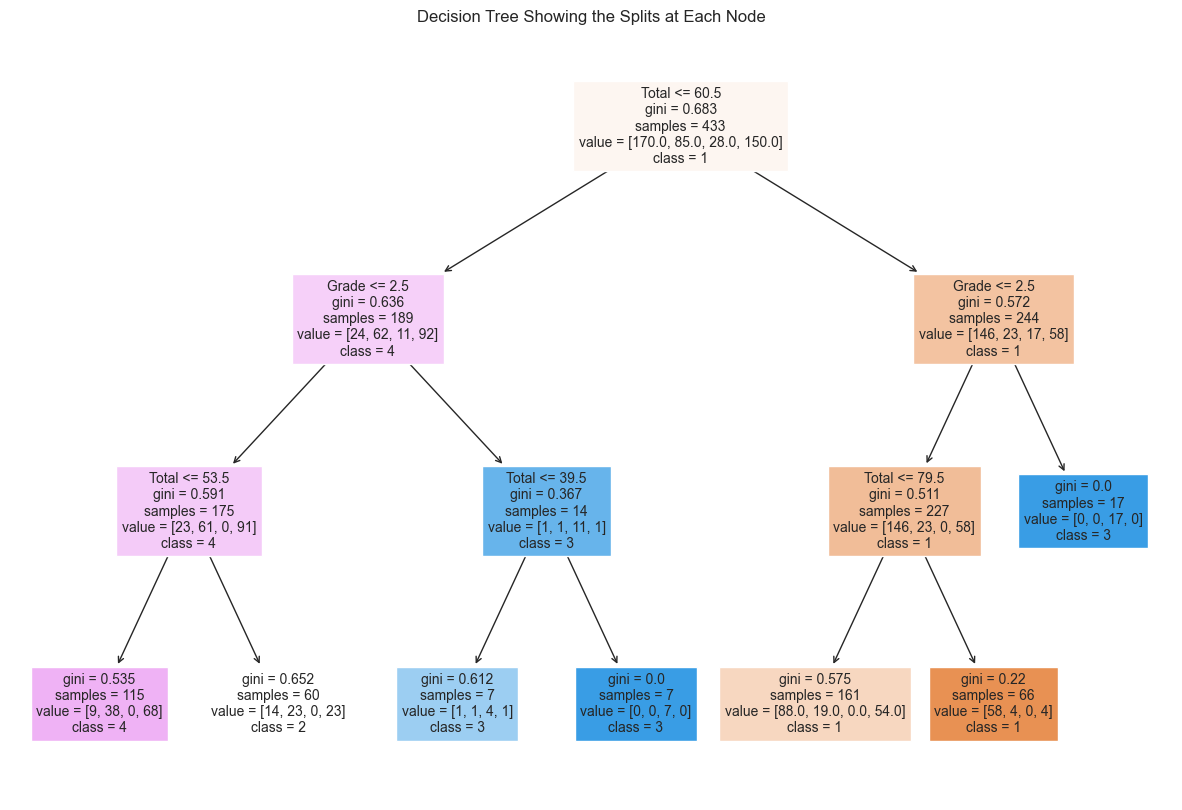
\includegraphics[scale=0.25]{./img/decision_tree.png}
    \caption{After balancing the results and performance, \textbf{the minimum number of samples to be split is 2, the minimum number of leaf samples is 5, and the optimal depth ranges from 3}. Although these three parameters can help to categorize different samples, if they are set to too large a value they may cause the tree structure to become too complex and cause overfitting.}
\end{figure}

% 决策树混淆矩阵
\begin{figure}[H]
    \centering % 使图片居中显示
    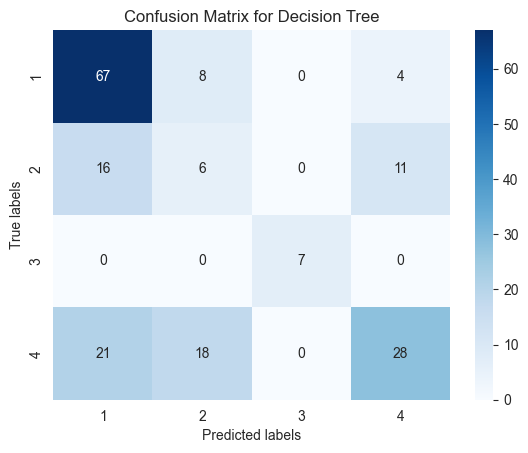
\includegraphics[scale=0.36]{./img/dt_matrix.png}
    \caption{Confusion matrix corresponding to Decision Tree classification results}
\end{figure}

\textbf{Fig.1} shows the decision tree image, sets an iterative process to judge the hyperparameter grid of the most suitable decision tree model, and finally selects the feature set composed of four features \textbf{[``Total'', ``Grade'', ``Q1'', ``Q4'']}, and sets the random state to 42. The re-cross-verification method obtained the \textbf{optimal F1 score of 0.5381, the accuracy is 0.5806}, and the final classification results were shown in the confusion matrix in \textbf{Fig.2}. 

% 随即森林多决策树
\subsection{Random Forest-Multiple Decision Tree}
Next, the random forest model is used to find out whether the results of the Programme category to which students belong can be predicted better than the results of a single decision tree through classification Settings in the multi-decision tree model.

Continue to use the best feature set of a single feature tree species \textbf{[``Total'', ``Grade'', ``Q1'', ``Q4'']}, set \textbf{the minimum sample split score to 10, the minimum number of leaf samples to 2 and the value range of the maximum depth to 10}, and the random state is set to 42. The \textbf{optimal F1 score was 0.6504, the accuracy is 0.6613}. The result is actually better than a single decision tree model, as in theory, because the random forest is able to build multiple decision trees, train them on different data, and ultimately decide the final result through a voting mechanism, so that even if some of the decision trees have problems with classification, other trees can help correct these mistakes.

% SVM
\section{Supportive Vector Machine}
Supportive Vector Machine (SVM) is a supervised learning algorithm for binary classification tasks. The main goal is to find an optimal decision boundary that maximizes the separation of different classes of samples. The decision boundary is determined by maximizing the margins between support vectors, which are the samples closest to the decision boundary. In this experiment, the \textbf{kernel function} is used as the kernel of the SVM model because the three datasets used are all high-dimensional datasets. Kernel functions can map samples to higher-dimensional feature Spaces to deal with linear non-fractional data sets.
% rbf公式
\begin{equation}
    K(x, x') = \exp\left(-\gamma \|x - x'\|^2\right)
\end{equation}
\textit{The rbf kernel is able to efficiently map the original feature space to a higher dimensional space, whereas the original dataset happens to be difficult to classify linearly, so this sub-linear mapping capability enables the data to be linearly classifiable after mapping to higher dimensions}
% svm混淆矩阵
\begin{figure}[H]
    \centering % 使图片居中显示
    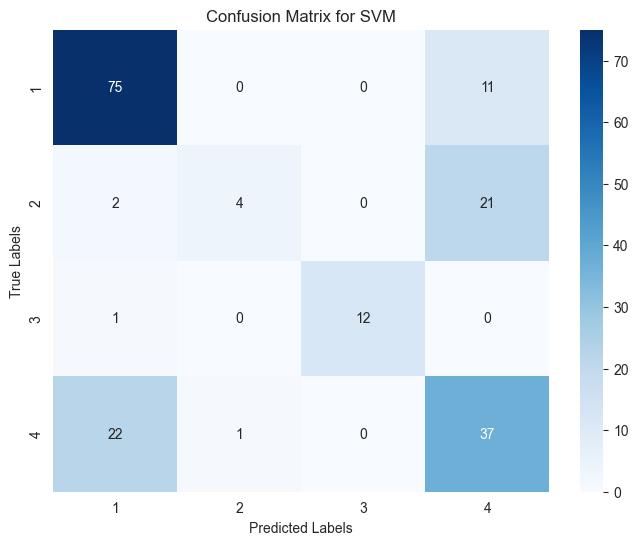
\includegraphics[scale=0.3]{./img/svm_matrix.png}
    \caption{Confusion matrix corresponding to svm classification results}
\end{figure}

Then there are two important hyperparameters in model training, which are \textbf{``C" and gamma}. C represents a regularization parameter that controls the trade-off between achieving larger margins and minimizing errors in training samples, and a larger C means that the penalty for misclassification is heavier and the model will be more inclined to classify all samples. In this experiment, \textbf{soft classification} will be selected, which allows a certain amount of error, so the classifier with stronger fault tolerance will be more extensive, so the value of C will be selected from a smaller number. At the same time,``gamma" determines the effect of a single sample, and here scale is chosen as gamma's choice. When a 4-dimensional feature set is selected and random state is set to 23 and \textbf{C to 5}, the \textbf{optimal F1 score is 0.6610, the accuracy is 0.6882}, and the classification results are shown in the confusion matrix in \textbf{Fig. 3}.

% 朴素贝叶斯
\section{Naive Bayes}
Naive Bayes is mainly the assumption of feature independence, that is, the assumption that each feature is independent of each other under the condition of class determination. This assumption greatly simplifies the calculation of the model, as it means that the joint probabilities can be decomposed into the product of individual probabilities.
% 朴素贝叶斯公式
\begin{equation}
    P(c|x) = \frac{P(x|c)P(c)}{P(x)}
\end{equation}

where \(P(c) \) is the prior probability of the category \(c \), \(P(x|c) \) is the probability of the feature \(x \) under the category \(c \), and \(P(x) \) is the marginal probability of the feature \(x \). In practice, in order to avoid underflow problems in calculations, it is common to take logarithms of these probabilities:
\begin{equation}
    \log P(c|x) = \log P(c) + \sum_{i=1}^n \log P(x_i|c) - \log P(x)
\end{equation}
% 朴素贝叶斯混淆矩阵
\begin{figure}[H]
    \centering % 使图片居中显示
    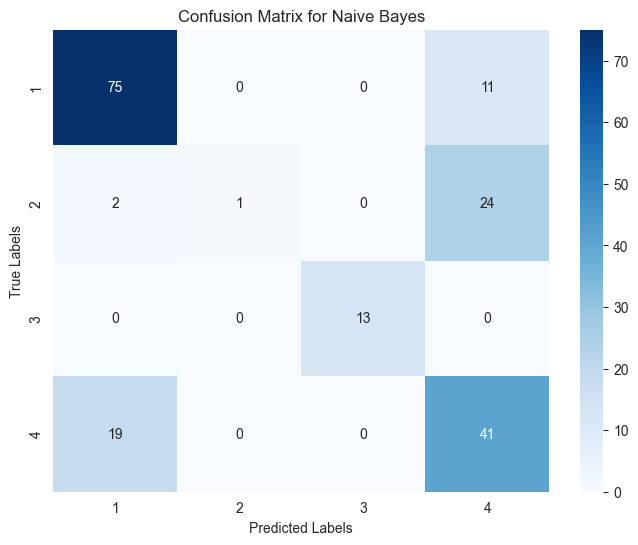
\includegraphics[scale=0.3]{./img/nb_matrix.png}
    \caption{Confusion matrix corresponding to Naive Bayes classification results}
\end{figure}

The final classification results are shown in the confusion matrix in \textbf{Fig. 4}. Again using the three feature sets above, and the random state is set to 23. After five-fold cross-validation, the final optimal classification results come from \textbf{[``Grade'', ``Total'', ``MCQ'', ``Q1'', ``Q2'', ``Q3'', ``Q4'', ``Q5'']}, and the \textbf{final F1 score of 0.6558, the accuracy is 0.6935}. It may be that there is no particularly strong direct relationship between test scores and student information, and thus fits the characteristics of naive Bayes' independent analysis of each feature.

% 集成学习
\section{Ensemble Learning}
% 集成学习图像
\begin{figure}[H]
    \centering % 使图片居中显示
    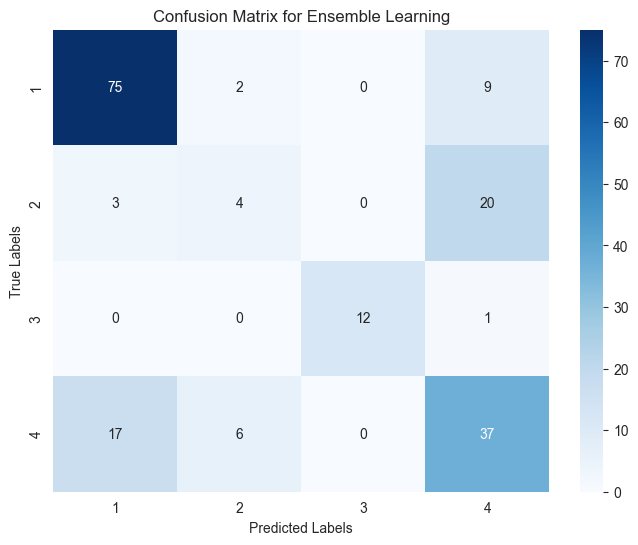
\includegraphics[scale=0.3]{./img/el_matrix.png}
    \caption{Confusion matrix corresponding to Ensemble Learning classification results}
\end{figure}

Ensemble learning integrates three basic classifiers: \textbf{decision tree}, \textbf{support vector machine (SVM)} and \textbf{naive Bayes}, feeds each classifier its feature set of optimal results, and then synthesizes the prediction probabilities of each classifier through \textbf{soft voting} mechanism to make the final decision. The consistency of the model input is ensured by training and testing with standardized processing data. The experimental results show that the \textbf{F1 score of this classification is 0.6680, the accuracy is 0.6882}, indicating that the integrated model can slightly improve the accuracy of classification compared with the single model.

% 总结
\section{Conclusion}
After comparing the results of various classifiers, \textbf{I think SVM may have better classification effect for such high-dimensional nonlinear divisible data}, because SVM has kernel function skills compared with other classifiers, and can map samples to high-dimensional space for division, thus solving the problem of linear indivisibility of current dimensions.

% % SVM决策边界
% \begin{figure}[H]
%     \centering % 使图片居中显示
%     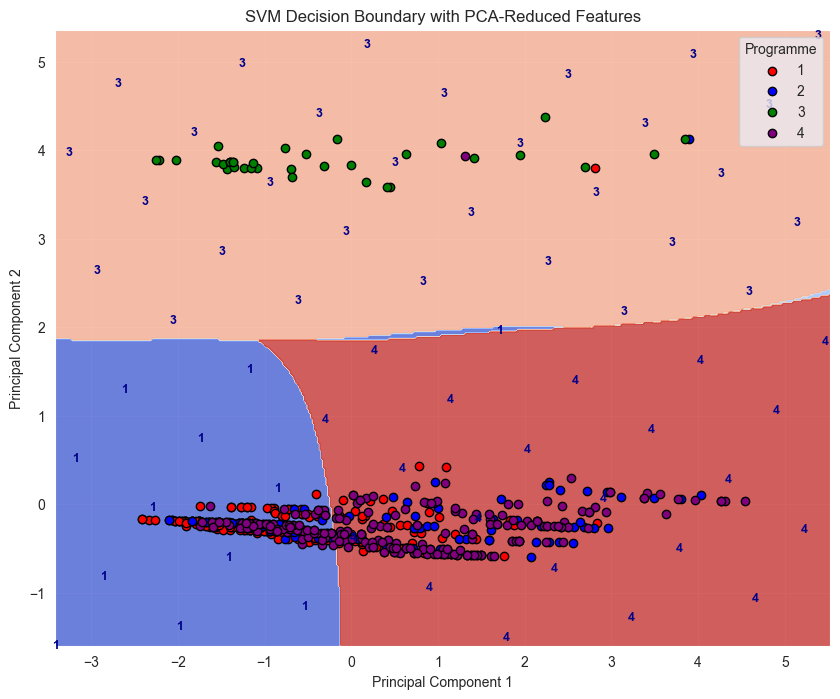
\includegraphics[scale=0.25]{./img/decision_boundary.png}
%     \caption{SVM Decision boundary}
% \end{figure}

% % ROC
% \begin{figure}[H]
%     \centering % 使图片居中显示
%     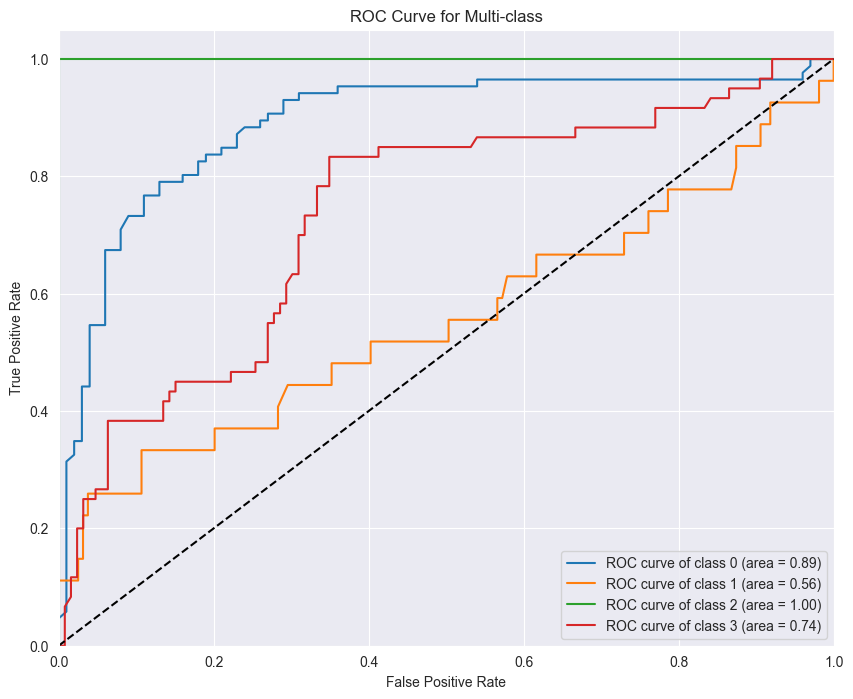
\includegraphics[scale=0.25]{./img/ROC.png}
%     \caption{SVM Receiver Operating Characteristic Graph}
% \end{figure}

\begin{figure}[H]
    \centering
    \begin{minipage}{0.23\textwidth}
        \centering
        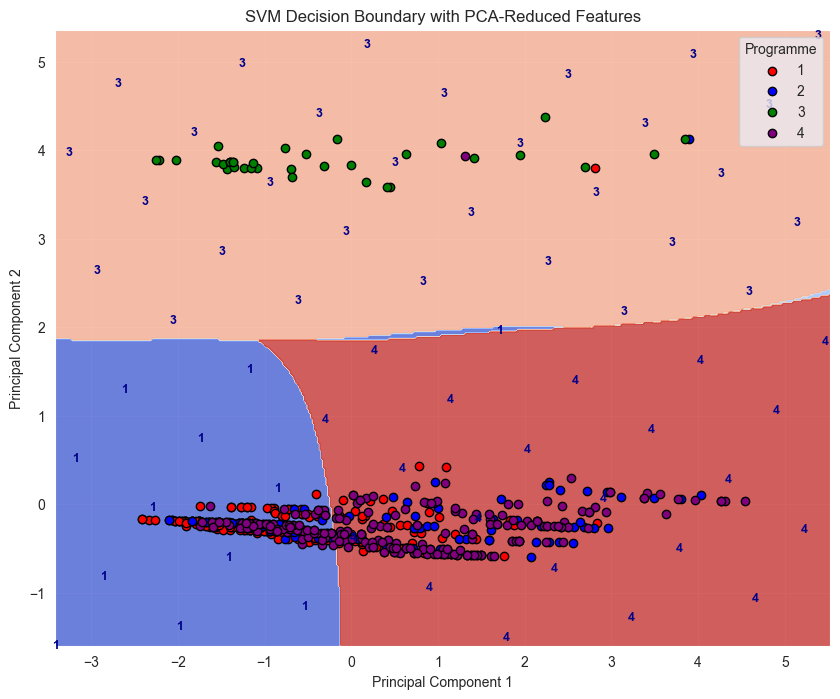
\includegraphics[width=\linewidth]{./img/decision_boundary.png}
        \caption{First Image}
        \label{SVM Decision Boundary}
    \end{minipage}
    % \hfill
    \begin{minipage}{0.23\textwidth}
        \centering
        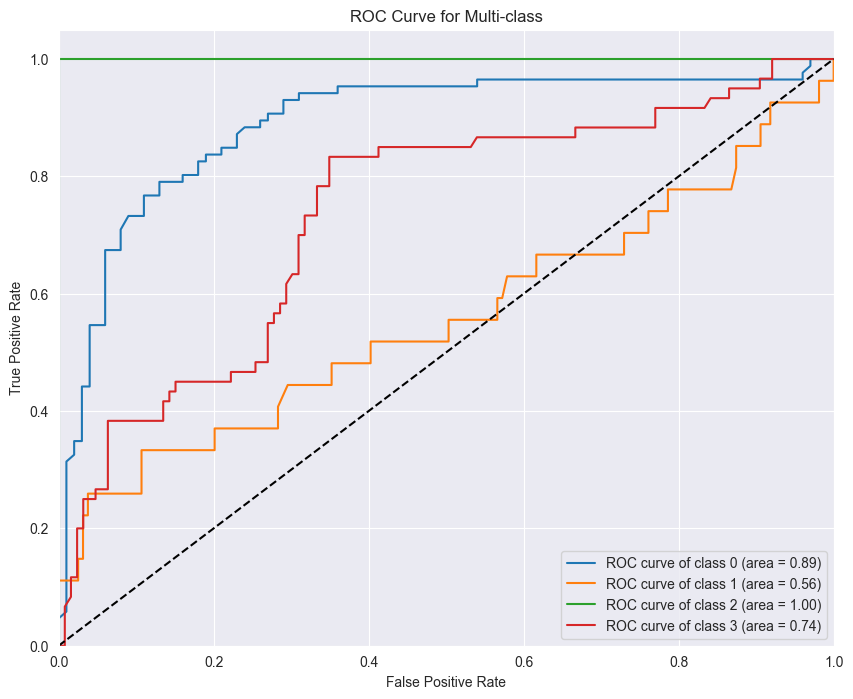
\includegraphics[width=\linewidth]{./img/ROC.png}
        \caption{ROC}
        \label{fig:sub2}
    \end{minipage}
\end{figure}

But in the end, it can be found that all the classifiers are unsatisfactory for the classification of Programme 2 and Programme 4. Even the best SVM can be seen by observing the 2-dimensional decision boundary division diagram \textbf{Fig. 5} and the Receiver Operating Characteristic (ROC) curve \textbf{Fig. 6}. After observing the 2-dimensional decision boundary division diagram Fig. 5 and the Receiver Operating Characteristic (ROC) curve Fig. 6, the SVM's classification effect on Programme2 and Programme4 in this experiment is also very poor. It may be that there is too little information about individual characteristics between the two, which makes it difficult for the classifier to clearly distinguish the relationship between the two. Can check code in \href{https://github.com/Gustav-Yellow/XJTLU-ICS/tree/main/INT104}{\color{blue} CW2}

\end{document}


